\documentclass{article}
\usepackage[margin=0.5in]{geometry}
\usepackage{graphicx}
\usepackage{subfigure}
\usepackage[colorlinks=true, linkcolor=blue]{hyperref} 
\usepackage{float}
%\usepackage{xcolor}


\begin{document}
\title{Predicting and classifying wines based on physical and chemical properties}
\maketitle
\begin{flushleft}
Wine is a \href{https://www.zionmarketresearch.com/report/wine-market}{circa \$300b industry}, and somewhat unique in the modern age; whilst most consumer goods are 
specified and produced in a controlled manner with \href{https://www.isixsigma.com/new-to-six-sigma/what-six-sigma/}{six sigma type methods}, 
wine varies significantly not just between brands, 
but between batches. 
\end{flushleft}
The question set is:
\\~\\
"Chemically speaking, what types of wine are there? What predicts wine quality?"
\\~\\
This question comes in two parts: the latter is more traditionally suited to regression techniques, 
the former appears little more towards neural net approaches, although testing for collinearity and bimodals
can still be of use.
\\~\\
The \href{http://archive.ics.uci.edu/ml/machine-learning-databases/wine-quality/}{dataset} consists of 6497 wines (1599 red, 4898 white) which have been assigned a quality rating (the dependent variable) from 0-10.  
10 (independent) variables have been measured: fixed and volatile acidity, citric acid levels, residual sugar, chlorides, free and total sulfur dioxide,
density, pH, sulphates and alcohol content (the dataset is complete, though units are not provided). 
\\~\\
On a superficial level, there are clearly two types of wine: red and white, although that may be considered anthropomorphic.  T-test of the two datasets
confirms they are indeed different in every measured variable except alcohol content, with red wines having greater acidity, less residual sugar, and less sulfur dioxide.

\begin{figure}[h]
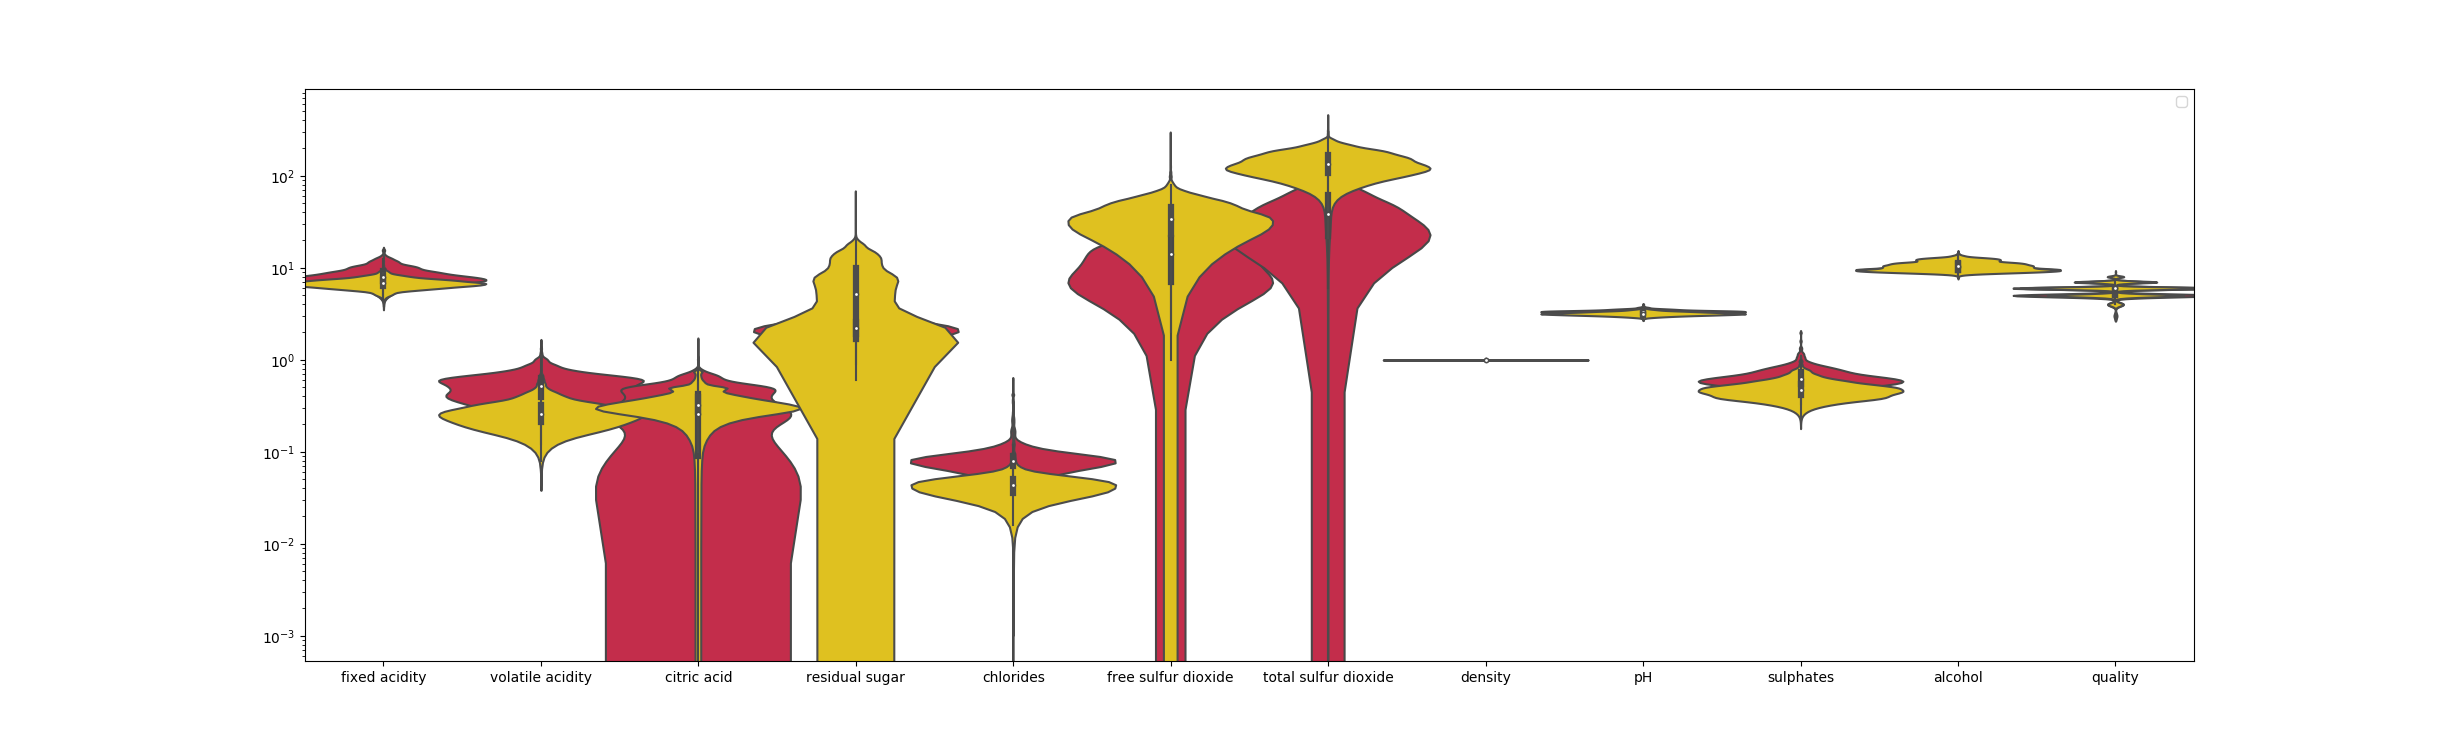
\includegraphics[width=\linewidth]{figures/red_white_properties_log_axis.png}
\caption{mean properties for red and white wines}
\label{fig:means}
\end{figure}

\section*{Types of wine}
llustrates correlation between different measured properties (darker colours indicate a greater association).  Some associations are intuitive; 
citric acid and fixed acidity are related, as are both with a low pH.  In addition, fixed acidity is associated with higher density, and 
chlorides with sulphates.

\begin{figure}[H]
\centering
\begin{subfigure}
  \centering
  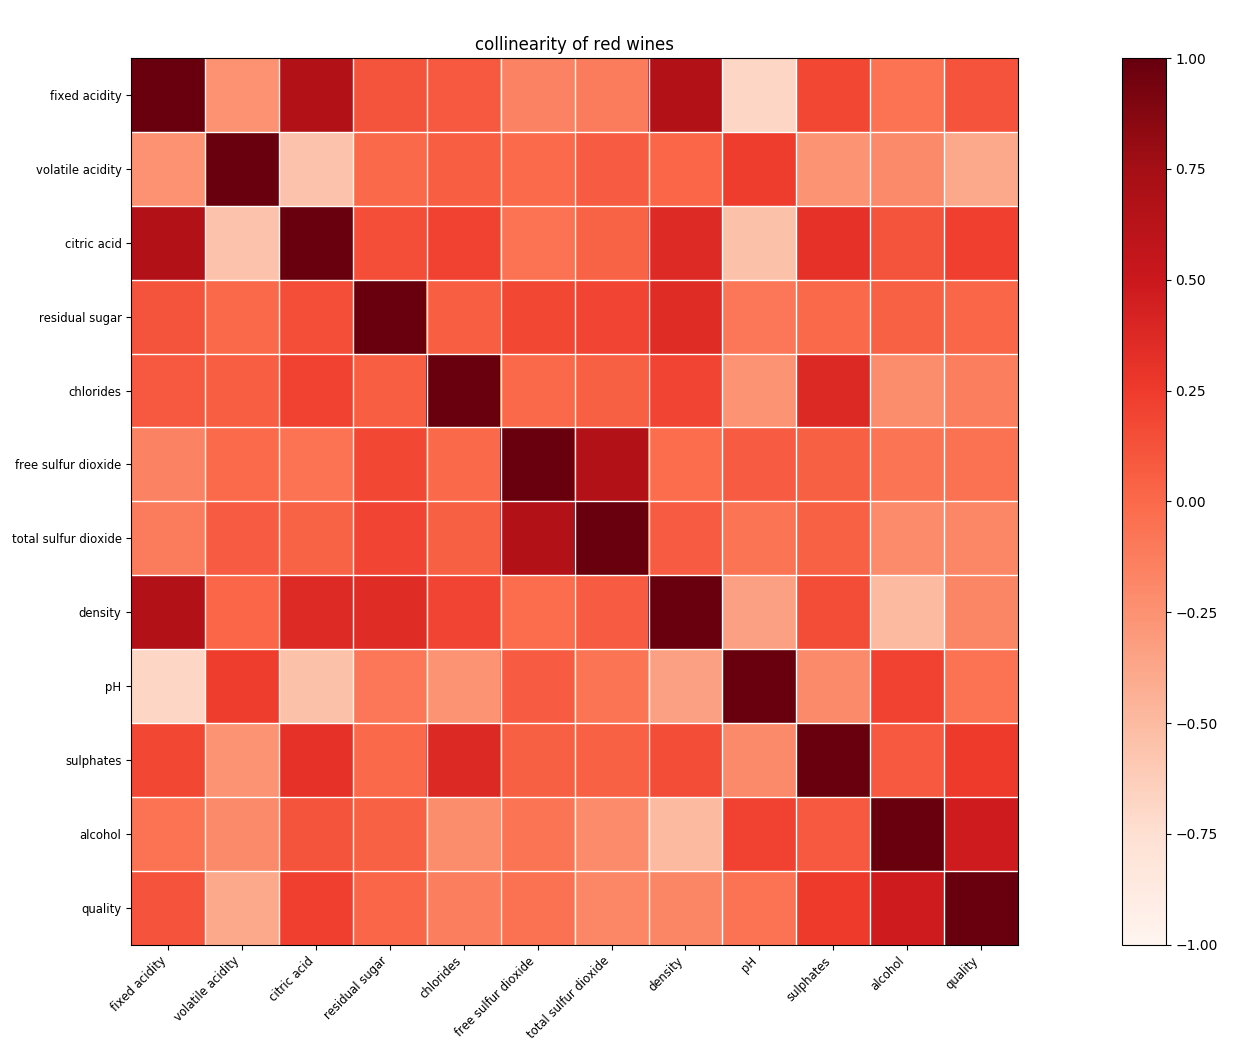
\includegraphics[width=0.4\linewidth]{figures/red_corr.png}
\end{subfigure}%
\begin{subfigure}
  \centering
  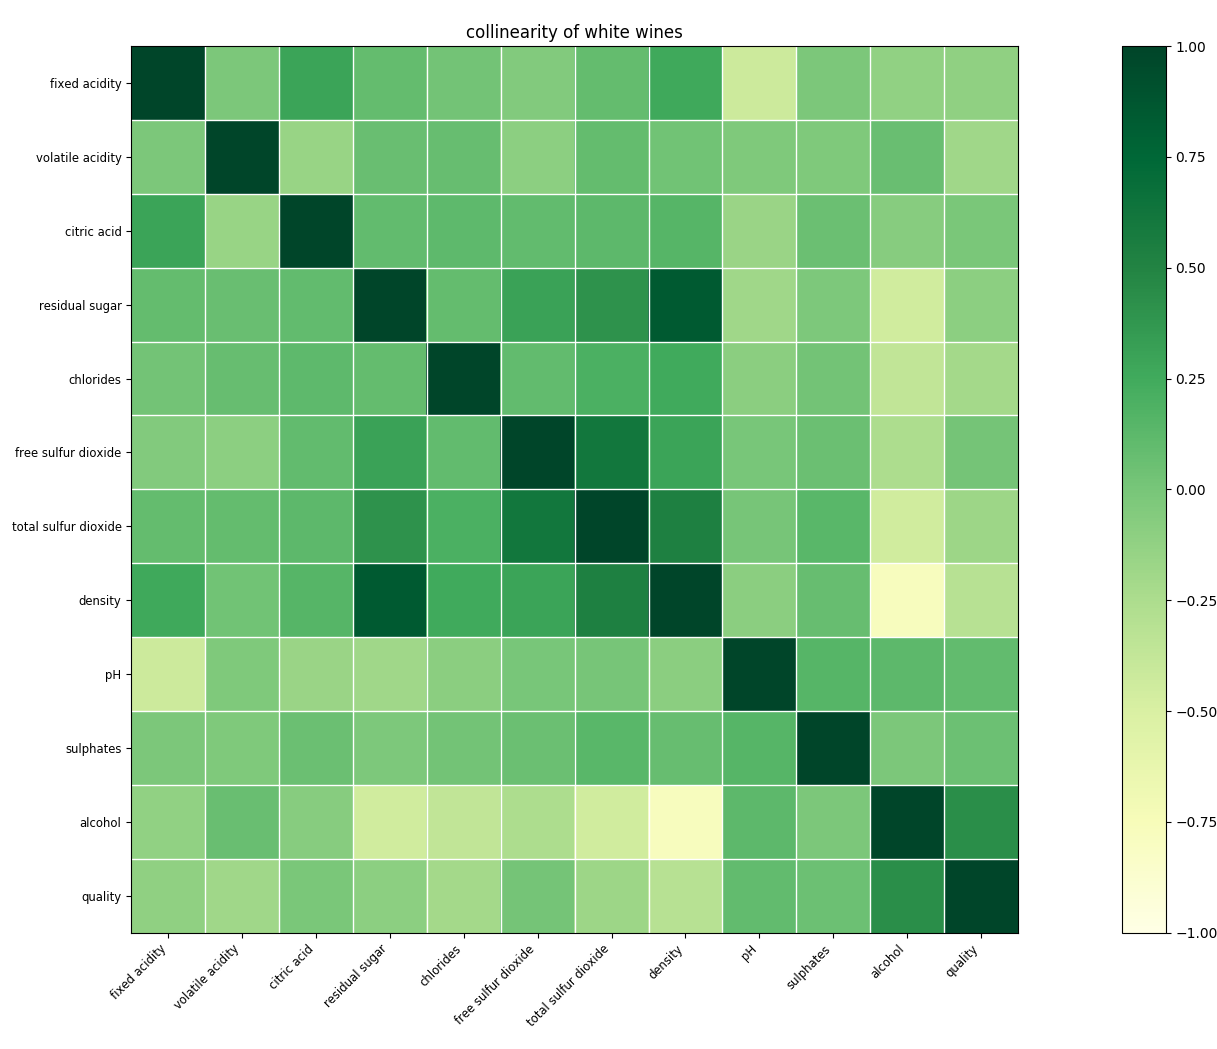
\includegraphics[width=0.4\linewidth]{figures/white_corr.png}
\end{subfigure}
\caption{associations between different wine properties}
\label{fig:correlations}
\end{figure}

\section*{Finding predictors}
It would be reasonable to assume that that winemakers have roughly optimised each chemical present, so that the optimum lies somewhere within the space 
tested: in this case a quadratic fit is appropriate.  It is equally possible that some quantities should simply be maximised.
\\~\\
Properties matching the stricter quadratic criteria are: for red wines, sulphates and citric acid; 
for white wines, free and total sulfur dioxide.  For red wine only, increasing alcohol content increased perceived quality ($\alpha < 0.01$).  
For both types, volatile acidity, chloride and density should be minimised.
\\~\\
Quality red wines (scoring 6 or higher) have on average significantly ($\alpha < 0.01$) lower volatile acidity, higher citric acid (and therefore lower pH),
higher sulphates, and higher alcohol, than poor reds (scoring 4 or lower).\linebreak
Quality white wines (scoring 6 or higher) have on average significantly ($\alpha < 0.01$) lower fixed and volatile acidity, higher residual sugar, chlorides, higher free sulfur dioxide but not total sulfur dioxide, density, than poor whites (scoring 4 or lower).\linebreak
Both scored higher for higher alcohol content.

\begin{figure}[h]
\centering
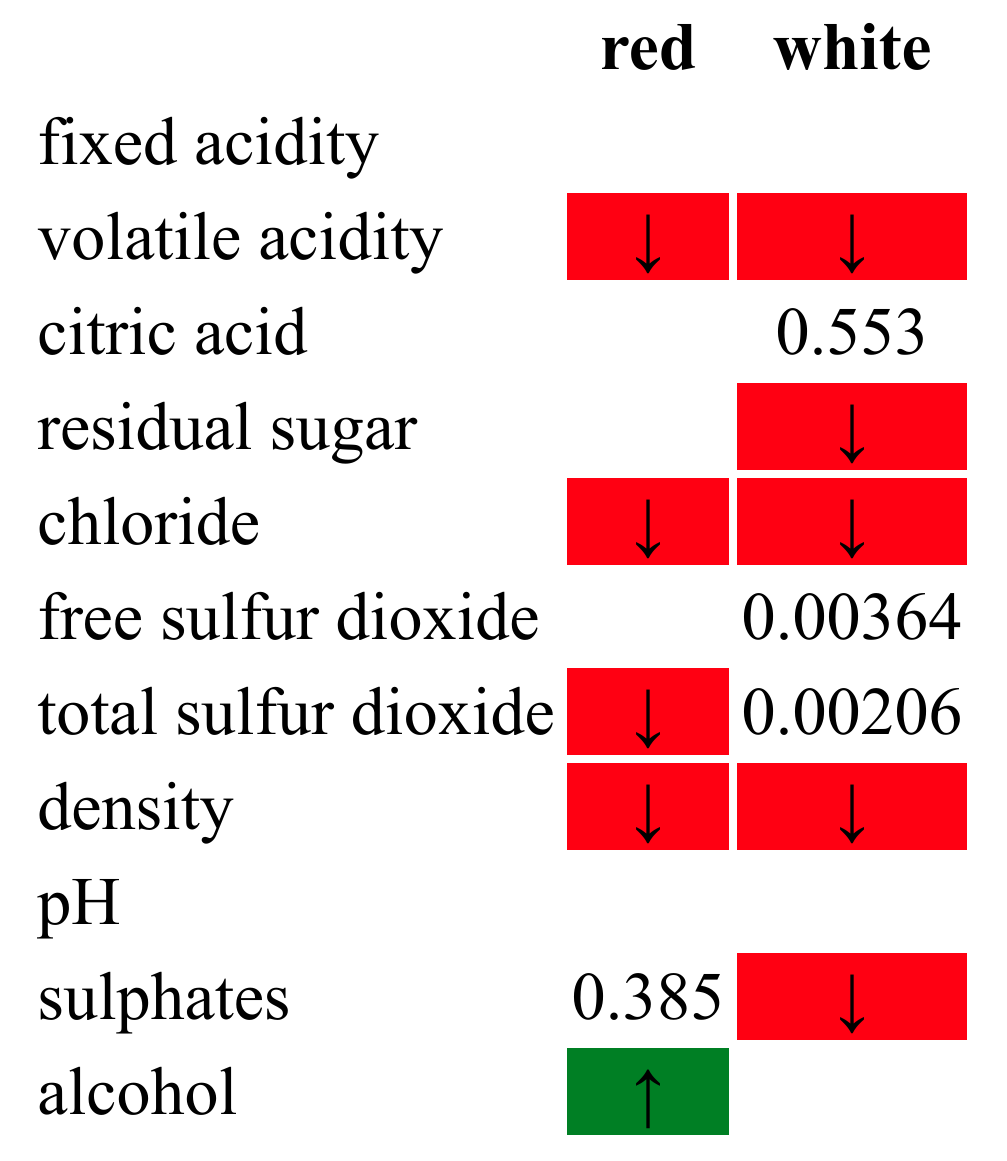
\includegraphics[height=5.0cm]{figures/recipe.png}
\caption{ideal properties for red and white wines; arrows indicate no optimum was found}
\label{fig:recipe}
\end{figure}


\end{document}
